\documentclass[a4paper, 11pt]{article}
%\usepackage[top=3cm, bottom=3cm, left = 2cm, right = 2cm]{geometry} 
%\geometry{a4paper}
\usepackage[utf8]{inputenc}
\usepackage{textcomp}
\usepackage{float}
\usepackage{graphicx}
\usepackage{parskip}
\usepackage{subfiles}
\usepackage{amsmath,amssymb}  
\usepackage{todonotes}
\usepackage[english]{babel}
\setlength {\marginparwidth }{2cm}
\usepackage{bm}  
\usepackage[pdftex,bookmarks,colorlinks,breaklinks]{hyperref}  
\hypersetup{linkcolor=black,citecolor=black,filecolor=black,urlcolor=black}
\usepackage{memhfixc} 
\usepackage{pdfsync}  
\usepackage{fancyhdr}
\pagestyle{fancy}
\setlength{\headheight}{14pt}
\bibliographystyle{plain}
\usepackage{listings}
\definecolor{backcolour}{RGB}{240,240,240}

\lstdefinestyle{mystyle}{
    backgroundcolor=\color{backcolour},   
    basicstyle=\ttfamily\tiny,
    breakatwhitespace=false,         
    breaklines=true,                 
    captionpos=b,                    
    keepspaces=true,                 
    showspaces=false,                
    showstringspaces=false,
    showtabs=false,                  
    tabsize=2,
	aboveskip=10pt, % set the space above the lstlisting block
	belowskip=10pt, % set the space below the lstlisting block
}
\lstset{style=mystyle}
\begin{document}

\begin{titlepage}
	\begin{center}
		
\includegraphics[scale=0.1]{images/unipd_logo.png}\\		
		\vspace{4\baselineskip}
		\Huge Real-time crowd information using Bluetooth: a full-stack solution\\
        \vspace{4\baselineskip}
		\Large Wireless Networks for Mobile Applications Exam Project\\
		\vfill
		Author: Marchiori Luca - 2090458\\
		AA: 2023-24\\

	\end{center}
\end{titlepage}


\tableofcontents

\newpage
\section{Introduction}
Understanding occupancy levels in buildings and rooms has become increasingly valuable in various contexts. One significant application is assessing the availability of seating in libraries that do not have booking systems in place. By knowing the number of people currently present in the library, individuals have a way of knowing the probability of finding an open space to study or work. 

But monitoring occupancy levels can also be crucial for effective workforce management: for businesses with multiple stores or offices, having real-time data on the number of people in each location allows management to allocate the appropriate amount of personnel accordingly. This ensures that staffing levels match customer demand or operational requirements, improving productivity and customer service.

In the event of a pandemic or other health-related concerns, understanding occupancy levels is critical for enforcing safety measures and organizing access to various places. By monitoring the number of individuals in a building or room, establishments can maintain social distancing protocols, manage crowd control, and implement measures to prevent overcrowding or potential outbreaks. Finally, in case of an emergency, it can be useful to get to know the amount of people in buildings to organize the rescue accordingly.

Tracking occupancy in buildings, especially those without strict entrance controls or booking systems, can indeed pose challenges. However, there are potential solutions to estimate occupancy even without exact tracking capabilities.

One approach could be leveraging the diffusion of Bluetooth technology in today's society. With most individuals carrying at least one device with Bluetooth capabilities, such as smartphones or other connected devices, a continuous Bluetooth scan can be conducted to estimate the number of devices present in a room. While this method may not provide an exact count of people, it can still offer a useful estimation and indicate the overall occupancy trends throughout the day. By calculating the average number of active Bluetooth devices carried by an individual, it becomes possible to estimate the number of people in an area. 

This project aims to develop a system that utilizes Bluetooth technology to display the approximate number of devices in a room over a certain period of time. The system would conduct continuous Bluetooth scans, tally the number of active devices, and present this data to provide insights into the occupancy patterns. By implementing such a system, organizations and individuals can have a better understanding of real-time occupancy levels, enabling them to make informed decisions about resource allocation, crowd management, and safety measures.

\section{System architecture}
The system architecture of the project is divided into two main units: the scanner devices and the server. The server itself is divided into a backend and a frontend applications.

The scanner devices are deployed as independent units. Each scanner consists of a single-board computer that performs periodic scans of the Bluetooth network, detecting all available devices within its range. Once the scanning routine is completed, the device sends the collected data to the backend of the centralized server via an HTTP POST request to a specific API endpoint.

The backend of the server functions as a web server. It receives the requests from the scanner devices, processes the data, and stores it into a database. Additionally, the backend handles GET requests from the frontend application: it retrieves the requested data by querying the database and provides it as a response to the frontend.

On the other hand, the server frontend serves as an interface between the user and the entire system. It provides webpages that can be accessed by users to interact with the system. The frontend can also trigger API requests to the backend server, requesting specific data. This data is then organized and presented to the user in a graphical view, enhancing the user experience.

This system architecture ensures that the scanner devices can operate autonomously, collecting data and sending it to the central server. The server backend handles data processing, storage, and retrieval, while the frontend enables user interaction and presentation of the collected data in a user-friendly manner. The following scheme (\ref{fig:system-architecture}) summarize the architecture and the data flow.

\begin{figure}
    \centering
    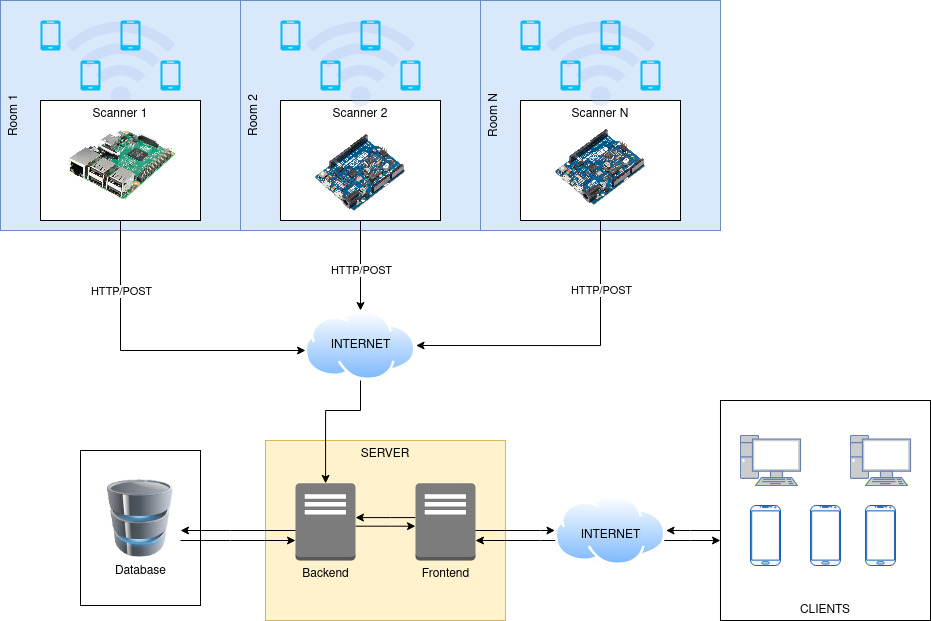
\includegraphics[width=1\linewidth]{images/WNMA-ProjectScheme.jpg}
    \caption{Project architecture}
    \label{fig:system-architecture}
\end{figure}


\section{Technologies}
\subsection{Hardware devices}
To implement the proposed system for tracking occupancy using Bluetooth scans, single-board computers like Raspberry Pi \cite{RPI} and Arduino \cite{arduino} are suitable choices. 

The devices used in this system need to have Bluetooth capabilities, allowing them to scan for nearby devices and gather occupancy data. Additionally, they should be capable of connecting to the internet either through WiFi or Ethernet to transmit the collected data to a server for storage and analysis. To facilitate the deployment process, these devices should be compact in size, making it easier to install them in various rooms and buildings and, considering the infrastructure cost, it is desirable to opt for inexpensive devices.

Both the Raspberry Pi and the Arduino, known for its versatility and functionality, fits the criteria effectively. They provides Bluetooth capabilities and options for internet connectivity through WiFi or Ethernet and their compact form factor allows for convenient deployment.

For this project due to board availability, a Raspberry Pi 3B+ has been used. However, since the logic is written in the Go programming language \cite{golang}, the exact same source code can be compiled with Tiny Go \cite{tinygo} \footnote{TinyGo is a Go compiler intended for use in small places such as microcontrollers, WebAssembly (wasm/wasi), and command-line tools.} to be run on Arduino or similar devices.

\subsection{Bluetooth}
Bluetooth is a wireless communication technology that allows devices to exchange data and connect with each other over short distances. It uses radio waves in the 2.4 GHz frequency range to establish a secure and low-power connection between devices.

Even though Bluetooth enables the sharing of data, in this project it is only used the scanning capabilities of this technology. When the scanner starts the discovery routine it sends out inquiry messages to discover other Bluetooth devices in its range. Bluetooth devices that receive the scan request can respond with their information, including their unique identifier known as MAC address. The scanning device can also measure the Received Signal Strength Indication (RSSI) of the responses that provides an estimate of the signal strength between the scanning device and the responding devices. This information can be used to estimate the proximity or distance between devices, or in this project can be used to exclude devices outside the room (or building). 

Bluetooth Low Energy (BLE) is a subset of Bluetooth designed for low-power applications. The main differences between Bluetooth and BLE are power consumption, data transfer rates, range, and application focus. Standard Bluetooth consumes more power, offers higher data transfer rates, has a longer range, and is suitable for continuous data streaming. BLE is optimized for low power consumption, has lower data transfer rates, has a shorter range, and is suitable for communication in devices with limited power resources. Both Bluetooth and BLE can coexist and support interoperability between devices.

This projects, using the go-bluetooth library, enables the scanning of both Bluetooth and Bluetooth Low Energy devices, allowing for scanning not only smartphones and computer but also smalls devices such as earphones, smart pencils, peripherals and watches.

\subsection{Programming languages and frameworks}
\subsubsection{Go}
Go, also known as Golang, is a compiled, statically typed, and open source programming language that has gained popularity for building microservices and cloud architectures. It is developed and mainteined by Google. In this project, both the server and the scanner logic are written in Go.

\textbf{Scanner}\\
One of the reasons for choosing Go for the scanner devices is its excellent run-time efficiency. It allows the scanner code to run smoothly even on low-power hardware like single board computers. Furthermore, Go can be compiled with the gc compiler to run on Linux with ARM processors, making it a suitable choice for devices like Raspberry Pi. Additionally, Go can be compiled with the tinygo compiler to run on embedded systems and microcontrollers such as Arduino.

To facilitate the interaction with Bluetooth devices on Linux systems, the go-bluetooth library \cite{go-bluetooth} has been used in this project. This library acts as a wrapper to the Bluez DBus API and offers high-level APIs that simplify the process of communicating with Bluetooth devices on Linux-based systems.

\textbf{Server}\\
For the server component of this project, Go was chosen due to its capability to support the development of web applications. The language provides a range of useful tools, including an integrated web server provided by the http package \cite{go-http} in its standard library. This allows to quickly set up and deploy web APIs that are used to receive data from scanners and provide data to the front end.

\subsubsection{React / JS}
React \cite{react} is a highly popular and widely used front-end JavaScript library that enables developers to build user interfaces based on reusable components. It is an open-source project maintained by Meta.

One of the key advantages of using React is its ability to create single-page applications, mobile applications, or server-rendered applications in conjunction with frameworks like Next.js. This flexibility allows developers to build applications for various platforms and use cases.

In this project, the frontend has been developed using React. By leveraging React's component-based architecture, it was possible to create reusable UI components that can be easily composed to build more complex user interfaces. This results in cleaner and more maintainable code and the possibility to easily expand the project with more features.

To implement the data visualization pages, the Apex Charts library \cite{apexcharts} has been used. This library provides powerful charting and graphing functionalities, allowing the presentation of data in a visually appealing and informative manner.

For handling API calls to the backend, the project uses the Axios library \cite{axios}. Axios simplifies the process of making HTTP requests and handling responses, providing a convenient and efficient way to interact with the backend server.

\subsection{Database}
The server implements SQLite \cite{sqlite} as its database system. SQLite belongs to the family of embedded databases, which are database management systems tightly integrated with an application software, avoiding the need for external servers. SQLite stores the database in files that can be easily managed and deployed, eliminating the need for complex server setups and heavier (DBMS). 
However, if this project will ever be deployed on a production enviroment, SQLite can be easily replaced with more powerful DBMS options such as MySQL or PostgreSQL, depending on the specific requirements and scalability needs of the project. These DBMSs offer additional features and can handle larger, more complex databases if necessary.

\section{Development}
\subsection{Scanner}
The scanner's main function consists on simply two task: run the Bluetooth device scan and posting the data to the back-end web server.

\begin{lstlisting}[language=Go]
func main() {
	log.Infof("Bluetooth affluence script started")
	aid := adapter.GetDefaultAdapterID()
	scan, err := Run(aid, 60) // The scan is 60 seconds long
	
	if err != nil {
		log.Error(err)
		os.Exit(1)
	}

	err = postScanResults(scan)
	if err != nil {
		log.Error("Error sending data to server")
		os.Exit(1)
	}

	os.Exit(0)
}

\end{lstlisting}

The length of the scanning process is hard-coded to 60 seconds. Using a scan duration too little can lead to not having enough time to scan all the devices around, setting it to a high value can lead to record devices that already left the room.

The scanning routine, given the Bluetooth adapter id, execute first a power cycle of the adapter to be use that it is up and running, after that, it flushes its cache to avoid missing devices, finally it runs the scan, until a timer-thread signals the expiration of the scan timeout. In the end, it fills a Scan datatype and sends it to the server.

The Scan datatype contains the list of the scanned devices, along with thier names, aliases, RSSIs, etc. along with the information of the scan such as the scanner properties and the timestamp of the scan.

In the following code block it's reported a simplified version of the code of the scanning function. Here, error handling and other functionalities are missing for space-related needs. The full code is available in the linked Github repository \cite{repo}. 


\begin{lstlisting}[language=Go]
func Run(adapterID string, timer int) (Scan, error) {
	var devices []Device
	a, err := adapter.GetAdapter(adapterID)
	var s Scanner = ScannerProps(*a)
	PowerCycle(*a)
	err = a.FlushDevices()
	discovery, cancel, err := api.Discover(a, nil)

	go func() {
		time.Sleep(time.Duration(timer) * time.Second)
		cancel()
	}()

	for ev := range discovery {
		dev, err := device.NewDevice1(ev.Path)
		device := Device{Address: dev.Properties.Address, Alias: dev.Properties.Alias, Name: dev.Properties.Name, RSSI: dev.Properties.RSSI, TxPower: dev.Properties.TxPower}
		device.Alias, device.Name)
		addDevice(&devices, device)
	}

	dt := time.Now().Format(time.RFC3339)
	scan := Scan{Devices: devices, Scanner: s, ScanTime: dt}
	return scan, nil
}

\end{lstlisting}

After the scanning function, the content of the Scan is converted into Json and sent to the back-end server with a POST request.

This script can be set to run automatically by configure an utility such as Crontab to execute the script. Crontab is a command in Unix-like operating systems that allows you to schedule recurring tasks or commands to run automatically at specific time intervals. The Crontab syntax consists of six fields, specifying the minute, hour, day of the month, month, day of the week, and the command to be executed. These fields can be set to specific values or can use special characters and wildcards to match multiple values. For example, the following Crontab entry executes the command "runScan" every 5 minutes:
\begin{lstlisting}[language=Bash]
*/5 * * * * /path/to/runScan
\end{lstlisting}

By increasing the frequency of the scan, it is possible to increase the granularity of the data store. Note that it can never be less than the scanning timeout set in the script.

\subsection{Server back-end}
The server backend is used to accomplish two tasks: storing the results sent by the scanner regarding the devices reached by a scan, storing them in the database, and providing the data to the client frontend upon request.

For the first part, an HTTP handler is defined to store the scanning information in a structure like the following:

\begin{lstlisting}[language=Go]
var input struct {
	Devices []struct {
		Address string `json:"address"`
		Name    string `json:"name"`
		Alias   string `json:"alias"`
		TxPower int16  `json:"txPower"`
		RSSI    int16  `json:"rssi"`
	}
	Scanner struct {
		Address string `json:"address"`
		Name    string `json:"name"`
		Alias   string `json:"alias"`
	}
	ScanTime string `json:"scanTime"`
}
\end{lstlisting}

By leveraging Go's tag feature, it is possible to automatically read the JSON in the HTTP body request and populate the input structure.

After that, the data is stored in the database with the following schema:(\ref{fig:database-schema}):

\begin{figure}
    \centering
    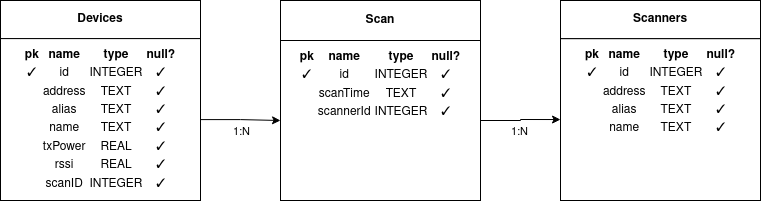
\includegraphics[width=1\linewidth]{images/WNMA_DB.drawio}
    \caption{Database schema}
    \label{fig:database-schema}
\end{figure}

The list of authorized scanner devices is stored in the database. When the scanner sends a new store request to the server, it is checked if it is among the authorized scanners. If it is, a new scan is stored to record the scanner ID and the time of the scan. For each scan, the information of the scanned devices is stored and associated with the scan. Alternatively, a more privacy-oriented and efficient solution would involve avoiding sending the list of scanned devices and only sending the count attribute.

To retrieve data from the server, a function that handles GET requests is defined. This function reads the start date, end date (the dates from and to which to retrieve the scanned devices), and the scanner ID. It is indeed possible to have multiple scanners and retrieve the data only for a certain scanner deployed in a specific room and a specific time range.

\begin{lstlisting}[language=Go]
func (app *application) countScanDevices(w http.ResponseWriter, r *http.Request) {
	w.Header().Set("Access-Control-Allow-Origin", "*")

	startDate := r.URL.Query().Get("start_date")
	endDate := r.URL.Query().Get("end_date")


	if startDate == "" || endDate == "" {
		app.errorResponse(w, r, http.StatusBadRequest, "Invalid date range")
		return
	}

	// Get the scanner id from the request
	scannerId, err := strconv.Atoi(r.URL.Query().Get("scanner_id"))
	if err != nil {
		app.logger.Error(err)
		app.errorResponse(w, r, http.StatusBadRequest, err.Error())
	}

	if scannerId == 0 {
		app.errorResponse(w, r, http.StatusBadRequest, "Invalid scanner id")
		return
	}
	
	[...]
	
\end{lstlisting}

The front-end will display a chart with the occupancy rate across the specified interval. Hence, after retrieving the data, the function will calculate, for every data point (every 5 minutes or depending on the scanner timeout), the total number of devices, the moving average of the devices, and the average number of devices present in the room for each time of the day.

The first piece of information that we can plot is the number of devices scanned for each time of the day. This can provide us with an idea of the real occupancy of the room, although it may show non-uniform numbers of devices due to devices being constantly included and excluded from the scan due to interferences and Bluetooth range. The following SQL query can retrieve the number of scanned devices for each time of the day:

\begin{lstlisting}[language=SQL]
	SELECT scan.scanTime, COUNT(devices.id) AS numDevices FROM scan
	LEFT JOIN devices ON scan.id = devices.scanID
	WHERE scan.scannerID = ?
	AND scan.scanTime BETWEEN ? AND ?
	GROUP BY scan.scanTime;
\end{lstlisting}

Moving average is a technique used in time series analysis that is particularly useful for smoothing out fluctuations and identifying trends in data. It involves calculating the average of a set of data points within a window or interval. This window moves along the data, incorporating new points and dropping old ones to create a series of average values.

After retrieving the data using the query above, it is possible to calculate the simple moving average as follows:

\begin{equation}
	{\displaystyle {\begin{aligned}{\textit {SMA}}_{k}&={\frac {p_{n-k+1}+p_{n-k+2}+\cdots +p_{n}}{k}}\\&={\frac {1}{k}}\sum _{i=n-k+1}^{n}p_{i}\end{aligned}}}
\end{equation}


\begin{lstlisting}[language=Go]
windowSize := 5
if len(results) >= windowSize {
	for i := windowSize - 1; i < len(results); i++ {
		sum := 0
		for j := i - (windowSize - 1); j <= i; j++ {
			sum += results[j].Count
			}
		results[i].Count = sum / windowSize
	}
}
\end{lstlisting}

Another interesting metric that can be calculated on the whole dataset, without specifying a date interval, is the Average value per timestamp, calculated on a 5-minute interval.

This metric allows us to estimate, on average, how many devices are in the room for each specific 5-minute interval (or any other interval depending on the scan rate).

To calculate this metric, we can write a SQL query similar to the one previously seen. This time, group the data by the 5-minute interval and count all devices present in that interval each day. Next, determine the exact size of the time interval (the number of days between the first and last datapoint) and divide the total device count by the number of days to obtain the mean value.

\begin{lstlisting}[language=SQL]
	SELECT strftime('%H:%M', scan.scanTime) AS minuteOfDay, COUNT(devices.id) AS averageValue
	FROM scan
	LEFT JOIN devices ON scan.id = devices.scanID
	WHERE scan.scannerID = ? AND scan.scanTime BETWEEN ? AND ?
	GROUP BY minuteOfDay;
\end{lstlisting}

\begin{lstlisting}[language=Go]
for rows.Next() {
	var scanTime string
	var numDevices int

	[...]
	res := scanDeviceAvg{scanTime, toFixed(float64(numDevices)/days, 2)}
	results = append(results, res)
}
\end{lstlisting}

The server is now ready to respond to fetch requests from the frontend. It will reply with the three metrics defined above so that the frontend can display them graphically. The full commented code, including the functions above, can be found in the project directory.

\section{Results}
The system has been tested using a single Raspberry Pi over 3 days at a local library. Due to the high cost of setting up a remote server for testing purposes, everything was configured to run on the Raspberry Pi using the loopback address. The scanner script runs every 5 minutes via Linux's crontab utility, and the backend server is active on port 4000. Every 5 minutes, the scanner conducts a bluetooth scan for approximately 60 seconds and sends the results to the backend server, which then stores them in the database.

By transferring the database and running the backend server on a PC alongside the frontend project, it is possible to analyze the recorded data and verify the overall functionality of the system.

\begin{figure}[H]
    \centering
    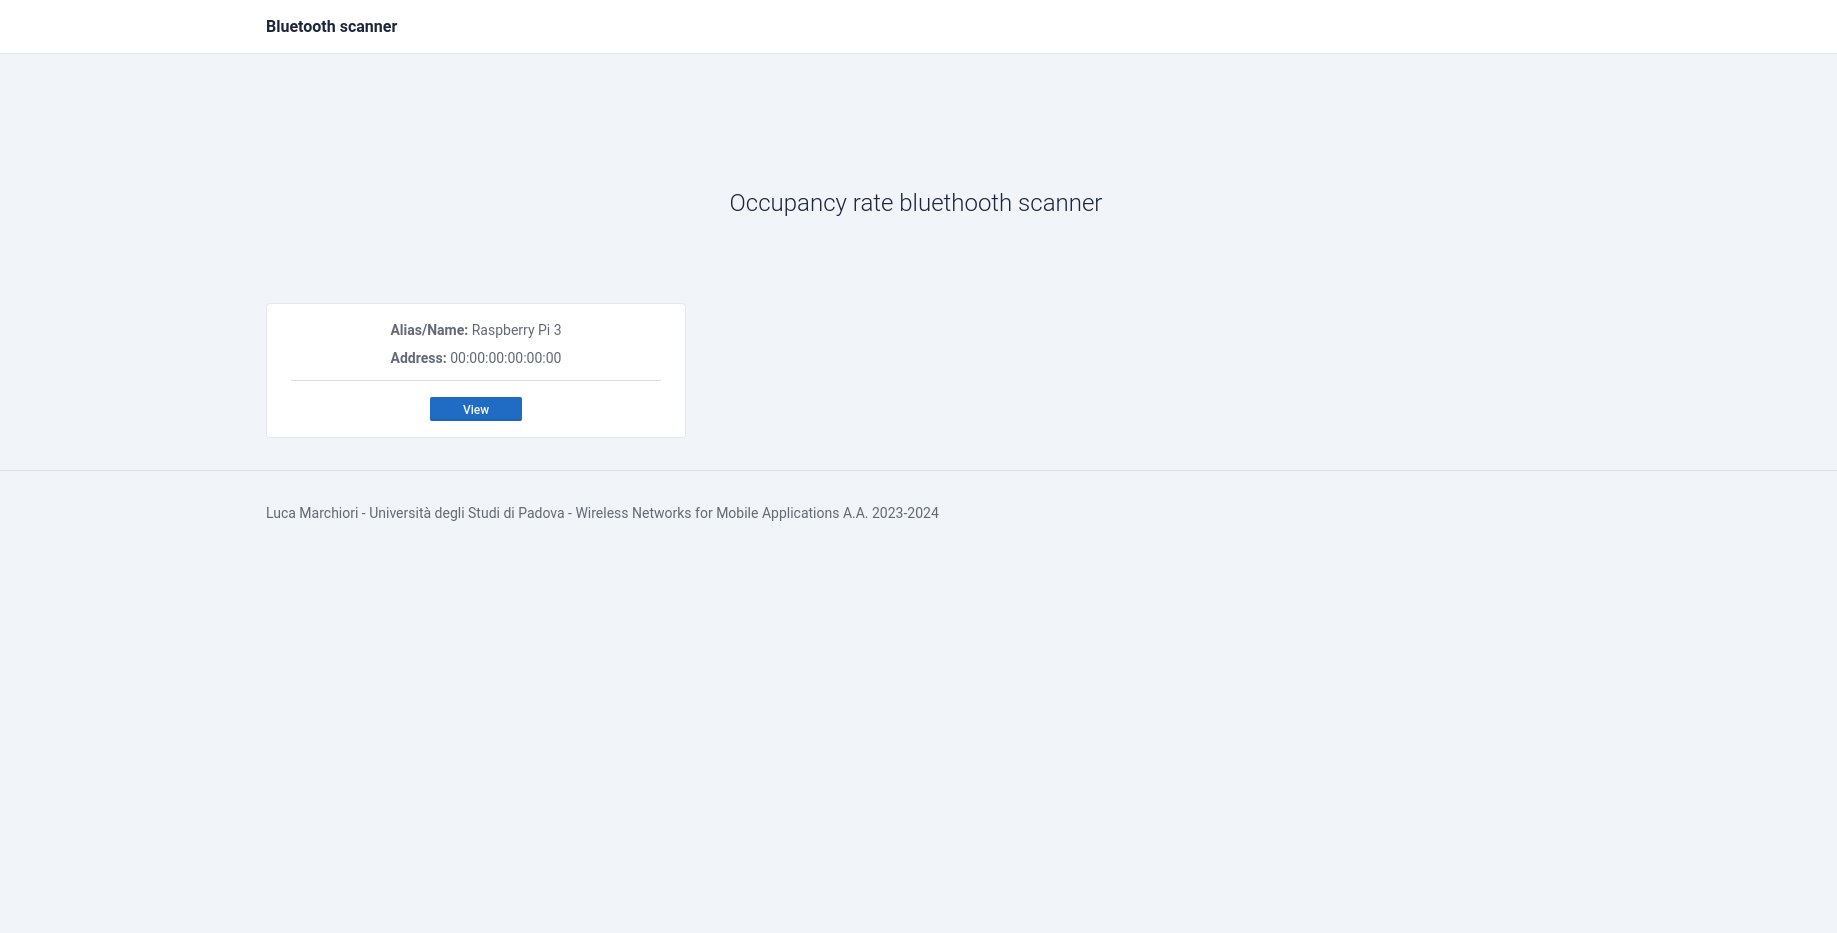
\includegraphics[width=1\linewidth]{images/DeviceIndexScreenshot.png}
    \caption{Web index}
    \label{fig:web-index}
\end{figure}

The first page displays a list of scanners. In cases where multiple scanners are used (such as one for each building or room), this page allows users to view the list of scanners. By clicking on a specific scanner, users can access a page where the recorded data is visualized.

\begin{figure}[H]
    \centering
    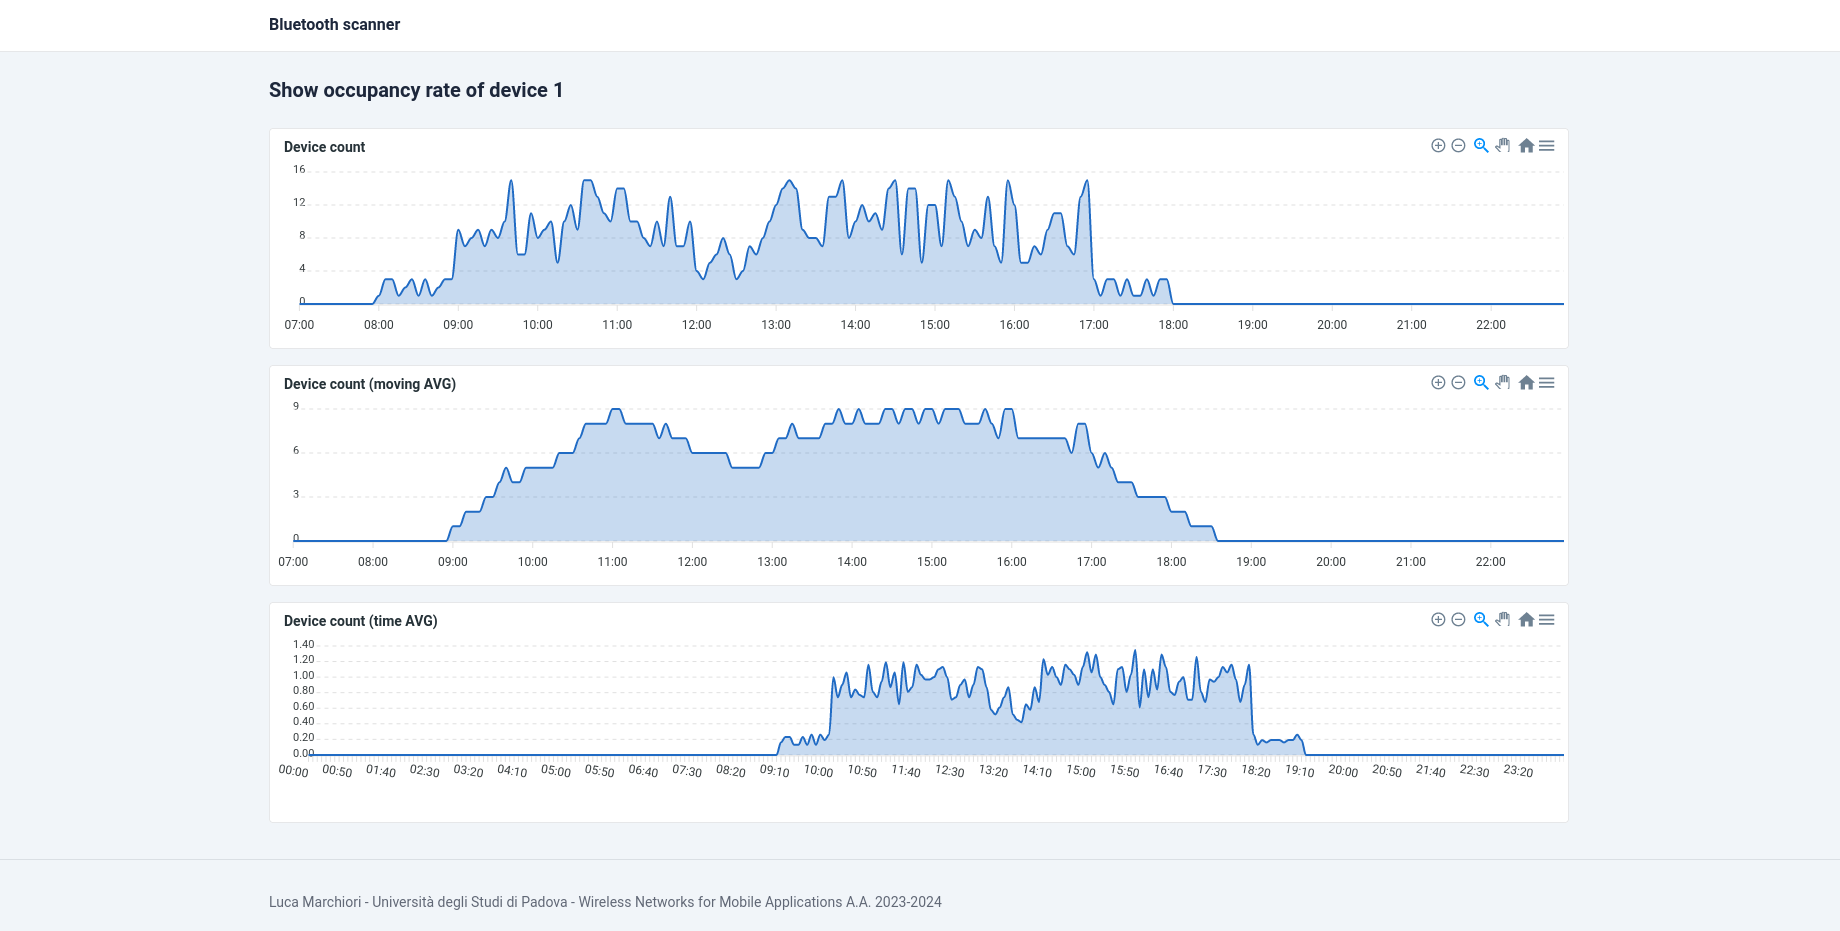
\includegraphics[width=1\linewidth]{images/DeviceShowScreenshot.png}
    \caption{Device count page}
    \label{fig:web-show}
\end{figure}

The first chart displays the simple device count. As mentioned in the backend description, the data points may show spikes caused by devices continuously entering and exiting the scan set due to Bluetooth reachability and interferences. By applying a moving average with a 25-minute window, the results can be smoothed out, enabling the detection of patterns in the data.

\begin{figure}[H]
    \centering
    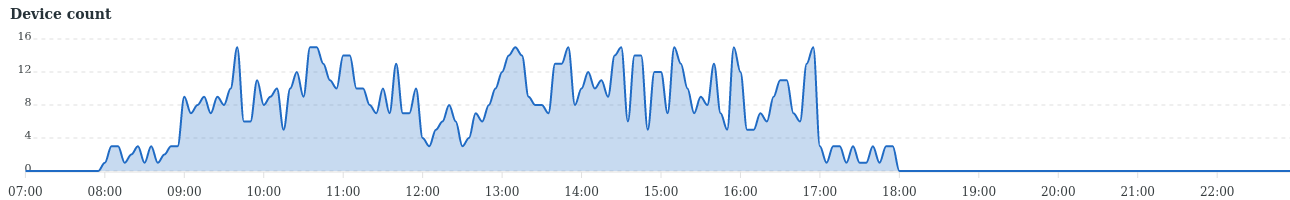
\includegraphics[width=1\linewidth]{images/c1wdhap3.png}
    \caption{Device count chart}
\end{figure}

\begin{figure}[H]
    \centering
    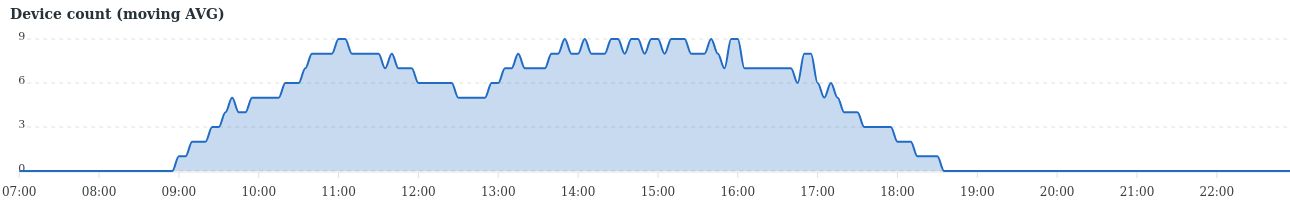
\includegraphics[width=1\linewidth]{images/tp0w3w99f.png}
    \caption{Device count with moving average}
\end{figure}

Here it is possible to see that the number of users increases from the opening time of the library (8.00) to around noon where many students probably leave the library for lunch. Here we can se a little decrease in the device count. In the afternoon there is again a small increment in the device count that finally starts to slowly go down to zero within the closing times of the library.

Here, it is possible to see that the number of users increases from the library's opening time (8:00) until around noon, when many students likely leave for lunch. This is reflected in a slight decrease in the device count. In the afternoon, there is a small increase in the device count, which slowly count down to zero by the library's closing time (18.00).

This data refers to a single day but the other days have more or less the same pattern. This can be seen using the average device count per timestamp, calculated on a 5-minute interval.

\begin{figure}[H]
    \centering
    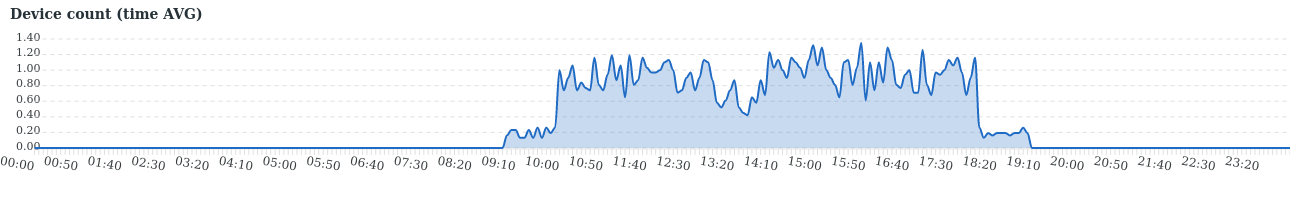
\includegraphics[width=1\linewidth]{images/reyw2zjfg.png}
    \caption{Average device count}
\end{figure}

\subsection{Conclusions}
The results appear to meet the initial requirements for understanding the occupancy rate patterns of people in the buildings. However, there are some considerations to take into account.

Associating a device's MAC address with an individual could potentially track their movements within rooms and buildings. It is then important to consider current privacy regulations as this software is capapble of getting logs of each Bluetooth device present in a building. To avoid this concern, the scanner could transmit only the total count of scanned devices to the software for each scan, instead of providing information on each individual device. In relation to this privacy issue, both Apple and Google have recently implemented Bluetooth MAC address randomization in their respective operating systems, iOS and Android. This technique ensures that the MAC addresses published by mobile devices in the search results can be randomized in order to avoid the possibility of fingerprinting the device. While this is not a problem related to counting the number of devices in the building, it can also help protect the privacy of users. However, it can be a challenge if the goal of systems like those described in this project is to track down the pattern of a specific user entering and exiting the buildings.

In regard to the test results, conducting tests on the system for only three days in a small library is not sufficient to gain a clear understanding of its effectiveness. The limited number of people entering and exiting the library leads to significant variations in the device count, highlighting the need for a longer testing period to validate the results. Additionally, inferring precise user numbers is challenging as it is impossible to determine how many Bluetooth devices individuals carry or if they have their Bluetooth enabled. The results can also vary greatly based on the type of environment being monitored. In settings like universities, people typically carry smartphones and computers, while some may also have smartwatches, earphones, and other Bluetooth-enabled devices leading to a high number of bluetooth device carried by each person. On the other hand, locations such as supermarkets or public offices may have many individuals without any Bluetooth devices. Moreover, in environments like companies or hospitals, there may be company-owned devices operating under Bluetooth that do not necessarily indicate the presence of individuals. This could result in a higher number of connected devices even during off-hours or when the building is unoccupied.

Therefore, there is a need for further testing of this system over an extended period and in different locations to compare the results and assess the system's effectiveness. It would also be beneficial to conduct surveys and studies to determine how many active Bluetooth devices individuals typically carry and how this may vary depending on factors such as location, age, and context.

From a technical perspective, the software architecture is functioning well and can be scaled up to accommodate more scanners for monitoring multiple rooms and buildings. The decoupling of components (scanner, frontend server, backend server) is a solid starting point for scalable software, allowing for the further development and expansion of each component to include additional features.


\newpage
\begin{thebibliography}{9}
\bibitem{repo}
Project's GitHub repository - \href{https://github.com/lucamarchiori/BluetoothAffluence}{github.com/lucamarchiori/BluetoothAffluence}
\bibitem{golang}
\href{https://go.dev/}{The Go Programming Language}

\bibitem{tinygo}
\href{https://tinygo.org/}{Tiny-Go - Go on embedded systems}

\bibitem{RPI}
\href{https://www.raspberrypi.com/documentation/computers/raspberry-pi.html}{Raspberry Pi}

\bibitem{arduino}
\href{https://docs.arduino.cc/}{Arduino}

\bibitem{go-bluetooth}
\href{https://pkg.go.dev/github.com/muka/go-bluetooth@v0.0.0-20221213043340-85dc80edc4e1#section-readme}{go-bluetooth Library}

\bibitem{go-http}
\href{https://pkg.go.dev/net/http}{Go HTTP package (std lib)}

\bibitem{react}
\href{https://react.dev/}{React framework}

\bibitem{apexcharts}
\href{https://apexcharts.com/}{Apex Chart JS charting library}

\bibitem{axios}
\href{https://axios-http.com/}{Axios - Promise based HTTP client}

\bibitem{sqlite}
\href{https://www.sqlite.org/index.html}{SQLite Database}
\end{thebibliography}
\end{document}